% Options for packages loaded elsewhere
\PassOptionsToPackage{unicode}{hyperref}
\PassOptionsToPackage{hyphens}{url}
\documentclass[
]{article}
\usepackage{xcolor}
\usepackage[margin=1in]{geometry}
\usepackage{amsmath,amssymb}
\setcounter{secnumdepth}{-\maxdimen} % remove section numbering
\usepackage{iftex}
\ifPDFTeX
  \usepackage[T1]{fontenc}
  \usepackage[utf8]{inputenc}
  \usepackage{textcomp} % provide euro and other symbols
\else % if luatex or xetex
  \usepackage{unicode-math} % this also loads fontspec
  \defaultfontfeatures{Scale=MatchLowercase}
  \defaultfontfeatures[\rmfamily]{Ligatures=TeX,Scale=1}
\fi
\usepackage{lmodern}
\ifPDFTeX\else
  % xetex/luatex font selection
\fi
% Use upquote if available, for straight quotes in verbatim environments
\IfFileExists{upquote.sty}{\usepackage{upquote}}{}
\IfFileExists{microtype.sty}{% use microtype if available
  \usepackage[]{microtype}
  \UseMicrotypeSet[protrusion]{basicmath} % disable protrusion for tt fonts
}{}
\makeatletter
\@ifundefined{KOMAClassName}{% if non-KOMA class
  \IfFileExists{parskip.sty}{%
    \usepackage{parskip}
  }{% else
    \setlength{\parindent}{0pt}
    \setlength{\parskip}{6pt plus 2pt minus 1pt}}
}{% if KOMA class
  \KOMAoptions{parskip=half}}
\makeatother
\usepackage{color}
\usepackage{fancyvrb}
\newcommand{\VerbBar}{|}
\newcommand{\VERB}{\Verb[commandchars=\\\{\}]}
\DefineVerbatimEnvironment{Highlighting}{Verbatim}{commandchars=\\\{\}}
% Add ',fontsize=\small' for more characters per line
\usepackage{framed}
\definecolor{shadecolor}{RGB}{248,248,248}
\newenvironment{Shaded}{\begin{snugshade}}{\end{snugshade}}
\newcommand{\AlertTok}[1]{\textcolor[rgb]{0.94,0.16,0.16}{#1}}
\newcommand{\AnnotationTok}[1]{\textcolor[rgb]{0.56,0.35,0.01}{\textbf{\textit{#1}}}}
\newcommand{\AttributeTok}[1]{\textcolor[rgb]{0.13,0.29,0.53}{#1}}
\newcommand{\BaseNTok}[1]{\textcolor[rgb]{0.00,0.00,0.81}{#1}}
\newcommand{\BuiltInTok}[1]{#1}
\newcommand{\CharTok}[1]{\textcolor[rgb]{0.31,0.60,0.02}{#1}}
\newcommand{\CommentTok}[1]{\textcolor[rgb]{0.56,0.35,0.01}{\textit{#1}}}
\newcommand{\CommentVarTok}[1]{\textcolor[rgb]{0.56,0.35,0.01}{\textbf{\textit{#1}}}}
\newcommand{\ConstantTok}[1]{\textcolor[rgb]{0.56,0.35,0.01}{#1}}
\newcommand{\ControlFlowTok}[1]{\textcolor[rgb]{0.13,0.29,0.53}{\textbf{#1}}}
\newcommand{\DataTypeTok}[1]{\textcolor[rgb]{0.13,0.29,0.53}{#1}}
\newcommand{\DecValTok}[1]{\textcolor[rgb]{0.00,0.00,0.81}{#1}}
\newcommand{\DocumentationTok}[1]{\textcolor[rgb]{0.56,0.35,0.01}{\textbf{\textit{#1}}}}
\newcommand{\ErrorTok}[1]{\textcolor[rgb]{0.64,0.00,0.00}{\textbf{#1}}}
\newcommand{\ExtensionTok}[1]{#1}
\newcommand{\FloatTok}[1]{\textcolor[rgb]{0.00,0.00,0.81}{#1}}
\newcommand{\FunctionTok}[1]{\textcolor[rgb]{0.13,0.29,0.53}{\textbf{#1}}}
\newcommand{\ImportTok}[1]{#1}
\newcommand{\InformationTok}[1]{\textcolor[rgb]{0.56,0.35,0.01}{\textbf{\textit{#1}}}}
\newcommand{\KeywordTok}[1]{\textcolor[rgb]{0.13,0.29,0.53}{\textbf{#1}}}
\newcommand{\NormalTok}[1]{#1}
\newcommand{\OperatorTok}[1]{\textcolor[rgb]{0.81,0.36,0.00}{\textbf{#1}}}
\newcommand{\OtherTok}[1]{\textcolor[rgb]{0.56,0.35,0.01}{#1}}
\newcommand{\PreprocessorTok}[1]{\textcolor[rgb]{0.56,0.35,0.01}{\textit{#1}}}
\newcommand{\RegionMarkerTok}[1]{#1}
\newcommand{\SpecialCharTok}[1]{\textcolor[rgb]{0.81,0.36,0.00}{\textbf{#1}}}
\newcommand{\SpecialStringTok}[1]{\textcolor[rgb]{0.31,0.60,0.02}{#1}}
\newcommand{\StringTok}[1]{\textcolor[rgb]{0.31,0.60,0.02}{#1}}
\newcommand{\VariableTok}[1]{\textcolor[rgb]{0.00,0.00,0.00}{#1}}
\newcommand{\VerbatimStringTok}[1]{\textcolor[rgb]{0.31,0.60,0.02}{#1}}
\newcommand{\WarningTok}[1]{\textcolor[rgb]{0.56,0.35,0.01}{\textbf{\textit{#1}}}}
\usepackage{graphicx}
\makeatletter
\newsavebox\pandoc@box
\newcommand*\pandocbounded[1]{% scales image to fit in text height/width
  \sbox\pandoc@box{#1}%
  \Gscale@div\@tempa{\textheight}{\dimexpr\ht\pandoc@box+\dp\pandoc@box\relax}%
  \Gscale@div\@tempb{\linewidth}{\wd\pandoc@box}%
  \ifdim\@tempb\p@<\@tempa\p@\let\@tempa\@tempb\fi% select the smaller of both
  \ifdim\@tempa\p@<\p@\scalebox{\@tempa}{\usebox\pandoc@box}%
  \else\usebox{\pandoc@box}%
  \fi%
}
% Set default figure placement to htbp
\def\fps@figure{htbp}
\makeatother
\setlength{\emergencystretch}{3em} % prevent overfull lines
\providecommand{\tightlist}{%
  \setlength{\itemsep}{0pt}\setlength{\parskip}{0pt}}
\usepackage{fvextra}
\DefineVerbatimEnvironment{Highlighting}{Verbatim}{commandchars=\\\{\},breaklines=true}
\usepackage{bookmark}
\IfFileExists{xurl.sty}{\usepackage{xurl}}{} % add URL line breaks if available
\urlstyle{same}
\hypersetup{
  pdftitle={Assignment\_2\_Data\_Wrangling\_Visualization},
  hidelinks,
  pdfcreator={LaTeX via pandoc}}

\title{Assignment\_2\_Data\_Wrangling\_Visualization}
\author{}
\date{\vspace{-2.5em}2026-09}

\begin{document}
\maketitle

\begin{Shaded}
\begin{Highlighting}[]
\CommentTok{\# Loading the packages I\textquotesingle{}ll use in this assignment}
\FunctionTok{library}\NormalTok{(tidyverse) }\CommentTok{\# Our primary data wrangling set of packages}
\end{Highlighting}
\end{Shaded}

\begin{verbatim}
## -- Attaching core tidyverse packages ------------------------ tidyverse 2.0.0 --
## v dplyr     1.2.1     v readr     2.2.0
## v forcats   1.0.1     v stringr   1.6.0
## v ggplot2   4.0.3     v tibble    3.3.1
## v lubridate 1.9.5     v tidyr     1.3.2
## v purrr     1.2.2     
## -- Conflicts ------------------------------------------ tidyverse_conflicts() --
## x dplyr::filter() masks stats::filter()
## x dplyr::lag()    masks stats::lag()
## i Use the conflicted package (<http://conflicted.r-lib.org/>) to force all conflicts to become errors
\end{verbatim}

\begin{Shaded}
\begin{Highlighting}[]
\FunctionTok{library}\NormalTok{(gridExtra) }\CommentTok{\# A package that helps arranging ggplot objects}
\end{Highlighting}
\end{Shaded}

\begin{verbatim}
## 
## Attaching package: 'gridExtra'
## 
## The following object is masked from 'package:dplyr':
## 
##     combine
\end{verbatim}

\begin{Shaded}
\begin{Highlighting}[]
\FunctionTok{library}\NormalTok{(ggpubr) }\CommentTok{\# For the statistical tests {-} Wilcoxon rank sum test}
\end{Highlighting}
\end{Shaded}

\begin{enumerate}
\def\labelenumi{\arabic{enumi})}
\tightlist
\item
  Generating random data is a useful skill. An exercise such as this is
  not only useful for developing data wrangling skills, but we can also
  use the resulting data for training and testing sets in machine
  learning. For this first exercise, I would like you to generate a data
  frame of random data with the following attributes:
\end{enumerate}

\begin{enumerate}
\def\labelenumi{\alph{enumi})}
\tightlist
\item
  The data frame should contain the following columns:
\end{enumerate}

\begin{itemize}
\tightlist
\item
  Participant\_ID: Generate reasonable participant IDs such as
  ``Participant\_001'', or something similar.
\item
  Sex: Male and Female
\item
  Age: Should follow a normal distribution and be bound between the ages
  18 and 90.
\item
  Activity\_Status: Should contain the levels ``Inactive'', ``Lightly
  Active'', ``Average Activity'', and ``Very Active''.
\item
  Disease\_Status: Should contain ``Case'' and ``Control'' levels.
  Participants with a systolic blood pressure greater than or equal to
  150 and a diastolic blood pressure greater than or equal to 95 should
  be considered a ``Case'', otherwise the participant should be
  considered a ``Control''.
\item
  Systolic\_Blood\_Pressure: The distribution from which the systolic
  blood pressure values should be taken is a normal distribution with a
  minimum of 110 and a maximum of 200. The mean should be 120 and the
  standard deviation should be 30.
\item
  Diastolic\_Blood\_Pressure: The diastolic blood pressures should be
  dependent on the systolic blood pressures if a systolic blood pressure
  is less than or equal to 120 than the diastolic blood pressure should
  follow a normal distribution where the minimum is 70 and the maximum
  is 100 with a mean of 80 and a standard deviation of 5. Otherwise, the
  diastolic blood pressure should have a minimum of 90 and a maximum of
  150. This should also follow a normal distribution. The mean should be
  100 abd the standard deviation should be 5.
\end{itemize}

\begin{enumerate}
\def\labelenumi{\alph{enumi})}
\setcounter{enumi}{1}
\tightlist
\item
  The data set should contain 100 participants
\end{enumerate}

\begin{Shaded}
\begin{Highlighting}[]
\DocumentationTok{\#\# Plan}
\CommentTok{\# 1. I\textquotesingle{}ll set my seed for the sampling, then I\textquotesingle{}ll set a number of participants to sample as a variable}
\CommentTok{\# 2. I\textquotesingle{}ll build a dataframe with all the variables that aren\textquotesingle{}t dependent on others. I\textquotesingle{}ll use rnorm and sample for the sampling as appropriate.}
\CommentTok{\# 3. I\textquotesingle{}ll mutate a variable categorizng the systolic blood pressure to above and below 120, then group by that variable so I can apply the different }
\CommentTok{\#    Diastolic blood pressure sampling distributions based on what group the participant falls into. }
\CommentTok{\# 4. Once I\textquotesingle{}ve grouped I\textquotesingle{}ll create a diastolic blood pressure variable, sampling based on group status as the instructions say to}
\CommentTok{\# 5. Then I\textquotesingle{}ll ungroup the data, and use the systolic value and the derived diastolic value to add the disease status value. }

\CommentTok{\# Set a seed for sample reproducibility}
\FunctionTok{set.seed}\NormalTok{(}\DecValTok{123}\NormalTok{)}

\CommentTok{\# The number of participants to sample}
\NormalTok{n }\OtherTok{\textless{}{-}} \DecValTok{100}  

\CommentTok{\# Generate random data}
\NormalTok{random\_data }\OtherTok{\textless{}{-}} \FunctionTok{data.frame}\NormalTok{(}
  \AttributeTok{Participant\_ID =} \FunctionTok{paste}\NormalTok{(}\StringTok{"pt"}\NormalTok{, }\DecValTok{1}\SpecialCharTok{:}\NormalTok{n, }\AttributeTok{sep =} \StringTok{"\_"}\NormalTok{),  }\CommentTok{\# Generate Subject IDs}
  \AttributeTok{Sex =} \FunctionTok{sample}\NormalTok{(}\FunctionTok{c}\NormalTok{(}\StringTok{"Male"}\NormalTok{, }\StringTok{"Female"}\NormalTok{), n, }\AttributeTok{replace =} \ConstantTok{TRUE}\NormalTok{),  }\CommentTok{\# Random sex values}
  \AttributeTok{Age =} \FunctionTok{pmax}\NormalTok{(}\DecValTok{18}\NormalTok{, }\FunctionTok{pmin}\NormalTok{(}\DecValTok{90}\NormalTok{, }\FunctionTok{round}\NormalTok{(}\FunctionTok{rnorm}\NormalTok{(n, }\AttributeTok{mean =} \DecValTok{50}\NormalTok{, }\AttributeTok{sd =} \DecValTok{10}\NormalTok{)))),  }\CommentTok{\# Random ages between 18 and 90}
  \AttributeTok{Activity\_Status =} \FunctionTok{sample}\NormalTok{(}\FunctionTok{c}\NormalTok{(}\StringTok{"Inactive"}\NormalTok{, }\StringTok{"Lightly Active"}\NormalTok{, }\StringTok{"Average Activity"}\NormalTok{, }\StringTok{"Very Active"}\NormalTok{), n, }\AttributeTok{replace =} \ConstantTok{TRUE}\NormalTok{),  }\CommentTok{\# Random activity status values}
  \AttributeTok{Systolic\_Blood\_Pressure =} \FunctionTok{pmax}\NormalTok{(}\DecValTok{110}\NormalTok{, }\FunctionTok{pmin}\NormalTok{(}\DecValTok{200}\NormalTok{, }\FunctionTok{round}\NormalTok{(}\FunctionTok{rnorm}\NormalTok{(n, }\AttributeTok{mean =} \DecValTok{120}\NormalTok{, }\AttributeTok{sd =} \DecValTok{30}\NormalTok{))))  }\CommentTok{\# Random systolic blood pressure values}
\NormalTok{) }\SpecialCharTok{\%\textgreater{}\%}
  \FunctionTok{mutate}\NormalTok{(}\AttributeTok{systolic\_group =} \FunctionTok{case\_when}\NormalTok{(}
\NormalTok{    Systolic\_Blood\_Pressure }\SpecialCharTok{\textless{}=} \DecValTok{120} \SpecialCharTok{\textasciitilde{}} \StringTok{"less\_120"}\NormalTok{, }\CommentTok{\# Create the grouping variable based on systolic BP}
\NormalTok{    Systolic\_Blood\_Pressure }\SpecialCharTok{\textgreater{}} \DecValTok{120} \SpecialCharTok{\textasciitilde{}} \StringTok{"gr\_120"}\NormalTok{,}
    \ConstantTok{TRUE} \SpecialCharTok{\textasciitilde{}} \ConstantTok{NA}
\NormalTok{  )) }\SpecialCharTok{\%\textgreater{}\%}
  \FunctionTok{group\_by}\NormalTok{(systolic\_group) }\SpecialCharTok{\%\textgreater{}\%} \CommentTok{\# Group by the new variable }
  \CommentTok{\# Execute the specific sampling pattern depending on the group the participant falls into}
  \FunctionTok{mutate}\NormalTok{(}
    \AttributeTok{Diastolic\_Blood\_Pressure =} \ControlFlowTok{if}\NormalTok{ (}\FunctionTok{cur\_group}\NormalTok{()}\SpecialCharTok{$}\NormalTok{systolic\_group }\SpecialCharTok{==} \StringTok{"less\_120"}\NormalTok{) \{}
      \FunctionTok{pmax}\NormalTok{(}\DecValTok{70}\NormalTok{, }\FunctionTok{pmin}\NormalTok{(}\DecValTok{100}\NormalTok{, }\FunctionTok{round}\NormalTok{(}\FunctionTok{rnorm}\NormalTok{(}\FunctionTok{n}\NormalTok{(), }\AttributeTok{mean =} \DecValTok{80}\NormalTok{, }\AttributeTok{sd =} \DecValTok{5}\NormalTok{))))}
\NormalTok{    \} }\ControlFlowTok{else}\NormalTok{ \{}
      \FunctionTok{pmax}\NormalTok{(}\DecValTok{90}\NormalTok{, }\FunctionTok{pmin}\NormalTok{(}\DecValTok{150}\NormalTok{, }\FunctionTok{round}\NormalTok{(}\FunctionTok{rnorm}\NormalTok{(}\FunctionTok{n}\NormalTok{(), }\AttributeTok{mean =} \DecValTok{100}\NormalTok{, }\AttributeTok{sd =} \DecValTok{5}\NormalTok{))))}
\NormalTok{    \} }\CommentTok{\# \#The diastolic blood pressures should be dependent on the systolic blood pressures if a systolic blood pressure is less than or equal to 120 than the diastolic blood pressure should follow a normal distribution where the minimum is 70 and the maximum is 100 with a mean of 80 and a standard deviation of 5. Otherwise, the diastolic blood pressure should have a minimum of 90 and a maximum of 150. This should also follow a normal distribution. The mean should be 100 abd the standard deviation should be 5.}
\NormalTok{  ) }\SpecialCharTok{\%\textgreater{}\%}
  \FunctionTok{ungroup}\NormalTok{() }\SpecialCharTok{\%\textgreater{}\%}
  \FunctionTok{mutate}\NormalTok{(}
    \AttributeTok{Disease\_Status =} \FunctionTok{case\_when}\NormalTok{( }\DocumentationTok{\#\# create the disease status variable based on BP values }
\NormalTok{      Systolic\_Blood\_Pressure }\SpecialCharTok{\textgreater{}=} \DecValTok{150} \SpecialCharTok{\&}\NormalTok{ Diastolic\_Blood\_Pressure }\SpecialCharTok{\textgreater{}=} \DecValTok{95} \SpecialCharTok{\textasciitilde{}} \StringTok{"Case"}\NormalTok{,}
      \ConstantTok{TRUE} \SpecialCharTok{\textasciitilde{}} \StringTok{"Control"}
\NormalTok{    ) }\CommentTok{\# Participants with a systolic blood pressure greater than or equal to 150 and a diastolic blood pressure greater than or equal to 95 should be considered a "Case", otherwise the participant should be considered a "Control".}
\NormalTok{  ) }\SpecialCharTok{\%\textgreater{}\%}
  \FunctionTok{select}\NormalTok{(}\SpecialCharTok{{-}}\NormalTok{systolic\_group) }\CommentTok{\# remove the grouping variable since it wasn\textquotesingle{}t asked for in the final dataset and is no longer needed}

\CommentTok{\# View the first few rows of the data}
\FunctionTok{head}\NormalTok{(random\_data)}
\end{Highlighting}
\end{Shaded}

\begin{verbatim}
## # A tibble: 6 x 7
##   Participant_ID Sex      Age Activity_Status Systolic_Blood_Pressure
##   <chr>          <chr>  <dbl> <chr>                             <dbl>
## 1 pt_1           Male      53 Lightly Active                      186
## 2 pt_2           Male      50 Lightly Active                      159
## 3 pt_3           Male      50 Inactive                            112
## 4 pt_4           Female    64 Lightly Active                      136
## 5 pt_5           Male      48 Inactive                            110
## 6 pt_6           Female    65 Inactive                            110
## # i 2 more variables: Diastolic_Blood_Pressure <dbl>, Disease_Status <chr>
\end{verbatim}

\begin{enumerate}
\def\labelenumi{\arabic{enumi})}
\setcounter{enumi}{1}
\tightlist
\item
  Convert the data frame you generated above from wide to long format
  based on the systolic and diastolic blood pressure columns. Make sure
  you take a look at the column names and how the data frame is now
  formatted after converting to long form!
\end{enumerate}

\begin{Shaded}
\begin{Highlighting}[]
\DocumentationTok{\#\# Plan}
\CommentTok{\# 1. I\textquotesingle{}ll use the tidyvere pivot\_longer() function to pivot on the two BP variables}

\NormalTok{long\_random\_data }\OtherTok{\textless{}{-}}\NormalTok{ random\_data }\SpecialCharTok{\%\textgreater{}\%}
  \FunctionTok{pivot\_longer}\NormalTok{(}
    \AttributeTok{cols =} \FunctionTok{c}\NormalTok{(Systolic\_Blood\_Pressure, Diastolic\_Blood\_Pressure), }\CommentTok{\# The 2 variables you want to pivot}
    \AttributeTok{names\_to =} \StringTok{"blood\_pressure\_type"}\NormalTok{, }\CommentTok{\# A new name for the columns}
    \AttributeTok{values\_to =} \StringTok{"blood\_pressure\_reading"} \CommentTok{\# A new name for the values}
\NormalTok{  )}

\CommentTok{\# View the first few rows of the data}
\FunctionTok{head}\NormalTok{(long\_random\_data)}
\end{Highlighting}
\end{Shaded}

\begin{verbatim}
## # A tibble: 6 x 7
##   Participant_ID Sex     Age Activity_Status Disease_Status blood_pressure_type 
##   <chr>          <chr> <dbl> <chr>           <chr>          <chr>               
## 1 pt_1           Male     53 Lightly Active  Case           Systolic_Blood_Pres~
## 2 pt_1           Male     53 Lightly Active  Case           Diastolic_Blood_Pre~
## 3 pt_2           Male     50 Lightly Active  Case           Systolic_Blood_Pres~
## 4 pt_2           Male     50 Lightly Active  Case           Diastolic_Blood_Pre~
## 5 pt_3           Male     50 Inactive        Control        Systolic_Blood_Pres~
## 6 pt_3           Male     50 Inactive        Control        Diastolic_Blood_Pre~
## # i 1 more variable: blood_pressure_reading <dbl>
\end{verbatim}

\begin{enumerate}
\def\labelenumi{\arabic{enumi})}
\setcounter{enumi}{2}
\tightlist
\item
  As Data Scientists, we will be asked to generate some neat looking
  figures. In the following questions, generate ggplot figures using the
  long format data you generated in the previous question, unless
  otherwise specified.
\end{enumerate}

\begin{enumerate}
\def\labelenumi{\alph{enumi})}
\tightlist
\item
  Generate a grouped ggplot2 box plot of the systolic and diastolic
  blood pressures in cases and controls. The x-axis should be the blood
  pressure types. The y-axis should be the blood pressure values. The
  fill should be the disease status: case or control.
\end{enumerate}

\begin{Shaded}
\begin{Highlighting}[]
\DocumentationTok{\#\# Plan}
\CommentTok{\# 1. use the ggplot function with geom\_boxplot() to build the boxplot with the prescribed x, y and fill using the long data }
\CommentTok{\# 2. add clear labels and title}
\CommentTok{\# 3. use theme\_minimal() to create a clean white background}
\CommentTok{\# 4. Add the Set1 color scheme for box plot fills}

\FunctionTok{ggplot}\NormalTok{(long\_random\_data, }\FunctionTok{aes}\NormalTok{(}\AttributeTok{x =}\NormalTok{ blood\_pressure\_type, }\AttributeTok{y =}\NormalTok{ blood\_pressure\_reading, }\AttributeTok{fill =}\NormalTok{ Disease\_Status)) }\SpecialCharTok{+} \CommentTok{\# Set variables to use}
  \FunctionTok{geom\_boxplot}\NormalTok{() }\SpecialCharTok{+} \CommentTok{\# Add type of plot}
  \FunctionTok{labs}\NormalTok{(}\AttributeTok{x =} \StringTok{"Blood Pressure Type"}\NormalTok{, }\AttributeTok{y =} \StringTok{"Blood Pressure Value"}\NormalTok{, }\AttributeTok{fill =} \StringTok{"Disease Status"}\NormalTok{, }
       \AttributeTok{title =} \StringTok{"Blood Pressure Readings }\SpecialCharTok{\textbackslash{}n}\StringTok{by Type and Disease Status"}\NormalTok{) }\SpecialCharTok{+} \CommentTok{\# Add labels and title}
  \FunctionTok{theme\_minimal}\NormalTok{() }\SpecialCharTok{+} \CommentTok{\# Create white background}
  \FunctionTok{scale\_fill\_brewer}\NormalTok{(}\AttributeTok{palette =} \StringTok{"Set1"}\NormalTok{) }\CommentTok{\# Add color scheme for fills}
\end{Highlighting}
\end{Shaded}

\pandocbounded{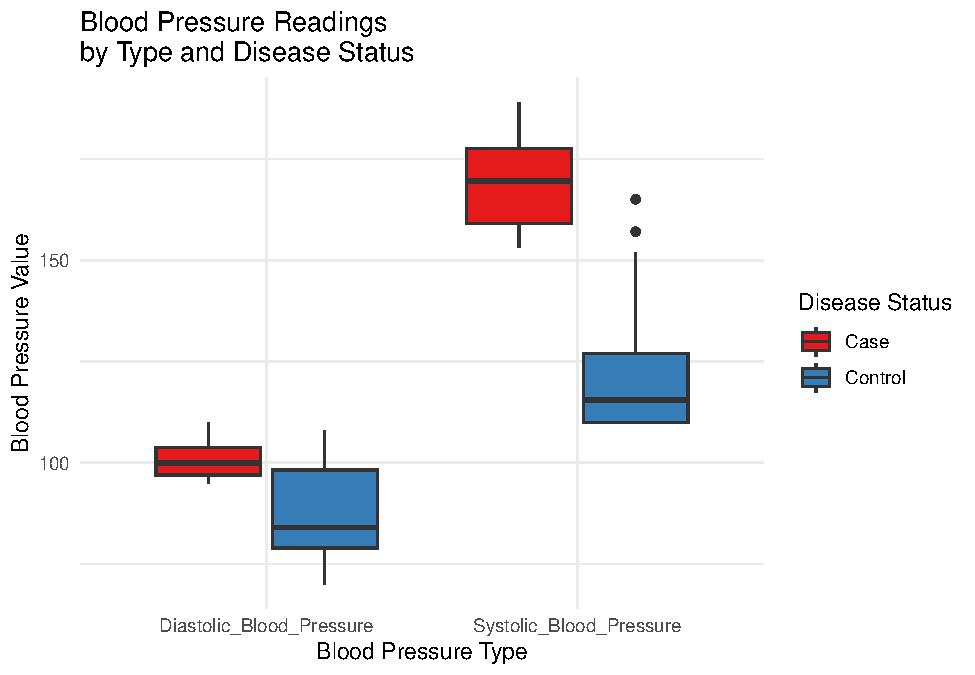
\includegraphics[keepaspectratio]{WeidnerSamuel-Assignment2_files/figure-latex/unnamed-chunk-3-1.pdf}}

\begin{enumerate}
\def\labelenumi{\alph{enumi})}
\setcounter{enumi}{1}
\tightlist
\item
  Generate a ggplot2 histogram of the systolic and diastolic blood
  pressures. Color the bars by disease status: case and control.
\end{enumerate}

\begin{Shaded}
\begin{Highlighting}[]
\DocumentationTok{\#\# Plan}
\CommentTok{\# 1. use the ggplot function with geom\_histogram() to build the histogram using the long data }
\CommentTok{\# 2. Set the x axis as blood pressure readings, the y axis will be count of frequency of observations with that reading}
\CommentTok{\# 3. Set the width to 5 so it is easier to read the chart}
\CommentTok{\# 4. Set other histogram parameters to standards better for visualizing}
\CommentTok{\# 5. add facet layer so there are two graphs for systolic and diastolic}
\CommentTok{\# 6. Add colors for fills of disease status}
\CommentTok{\# 7. use theme\_minimal() to create a clean white background}
\CommentTok{\# 8. add some more formatting}
\CommentTok{\# 4. Add labeling and titling}

\FunctionTok{ggplot}\NormalTok{(long\_random\_data, }\FunctionTok{aes}\NormalTok{(}\AttributeTok{x =}\NormalTok{ blood\_pressure\_reading, }\AttributeTok{fill =}\NormalTok{ Disease\_Status)) }\SpecialCharTok{+}
  \CommentTok{\# Histogram parameters}
  \FunctionTok{geom\_histogram}\NormalTok{(}
    \AttributeTok{binwidth =} \DecValTok{5}\NormalTok{,           }\CommentTok{\# Each bin contains a range of 5 different integer readings}
    \AttributeTok{alpha =} \FloatTok{0.6}\NormalTok{,            }\CommentTok{\# Makes overlap in bars see{-}through}
    \AttributeTok{position =} \StringTok{"identity"}\NormalTok{,  }\CommentTok{\# Keeps bars independent but on top of each other (which is why the overlap being see{-}through matters)}
    \AttributeTok{color =} \StringTok{"white"}         \CommentTok{\# Add a border separating bars next to each other so it\textquotesingle{}s easier to see}
\NormalTok{  ) }\SpecialCharTok{+}
  \CommentTok{\# Facet layer (split the plot into two panels for Systolic and Diastolic)}
  \CommentTok{\# scales = "free" allows the axes to adjust to fit each test type value range}
  \FunctionTok{facet\_wrap}\NormalTok{(}\SpecialCharTok{\textasciitilde{}}\NormalTok{ blood\_pressure\_type, }\AttributeTok{scales =} \StringTok{"free"}\NormalTok{, }\AttributeTok{ncol =} \DecValTok{2}\NormalTok{) }\SpecialCharTok{+}
  \CommentTok{\# Color Customizing}
  \FunctionTok{scale\_fill\_manual}\NormalTok{(}
    \AttributeTok{values =} \FunctionTok{c}\NormalTok{(}
      \StringTok{"Case"}      \OtherTok{=} \StringTok{"\#1f77b4"}\NormalTok{, }\CommentTok{\# Blue}
      \StringTok{"Control"}  \OtherTok{=} \StringTok{"\#ff7f0e"}  \CommentTok{\# Orange}
\NormalTok{    )}
\NormalTok{  ) }\SpecialCharTok{+}
  \FunctionTok{theme\_minimal}\NormalTok{() }\SpecialCharTok{+}
  \FunctionTok{theme}\NormalTok{(}
    \AttributeTok{legend.position =} \StringTok{"bottom"}\NormalTok{,          }\CommentTok{\# put the disease status legend at the bottom}
    \AttributeTok{strip.text =} \FunctionTok{element\_text}\NormalTok{(}\AttributeTok{face=}\StringTok{"bold"}\NormalTok{) }\CommentTok{\# bold "Systolic" and "Diastolic" labels}
\NormalTok{  ) }\SpecialCharTok{+}
  \CommentTok{\# Labels}
  \FunctionTok{labs}\NormalTok{(}
    \AttributeTok{title =} \StringTok{"Distribution of Blood Pressure Measurements by Disease Status"}\NormalTok{,}
    \AttributeTok{x =} \StringTok{"Blood Pressure"}\NormalTok{,}
    \AttributeTok{y =} \StringTok{"Frequency / Count"}\NormalTok{,}
    \AttributeTok{fill =} \StringTok{"Disease Status"}
\NormalTok{  )}
\end{Highlighting}
\end{Shaded}

\pandocbounded{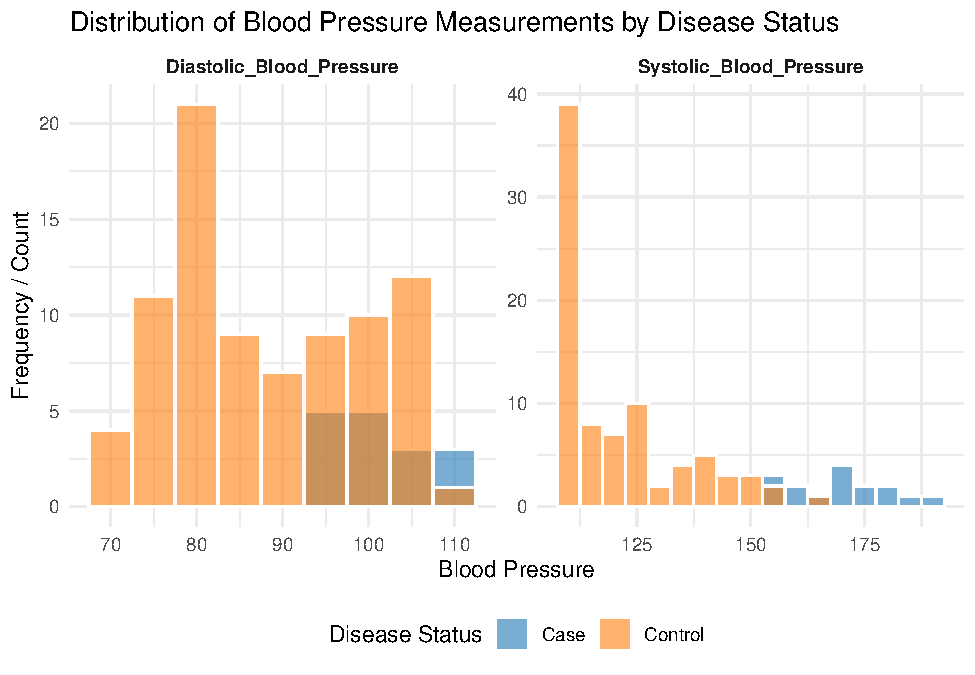
\includegraphics[keepaspectratio]{WeidnerSamuel-Assignment2_files/figure-latex/unnamed-chunk-4-1.pdf}}

\begin{enumerate}
\def\labelenumi{\alph{enumi})}
\setcounter{enumi}{2}
\tightlist
\item
  Using the wide format data frame, generate a scatter plot of systolic
  blood pressure on the x-axis and diastolic blood pressure on the
  y-axis. Once again, color the points by disease status: case and
  control.
\end{enumerate}

\begin{Shaded}
\begin{Highlighting}[]
\DocumentationTok{\#\# Plan }
\CommentTok{\# 1. use the ggplot function with geom\_point() to build the histogram using the wide data}
\CommentTok{\# 2. Plot the two blood pressure types on the x and y axis as requested}
\CommentTok{\# 3. Add a layer to add color to the points based on disease status}
\CommentTok{\# 4. use theme\_minimal() for a white background}

\FunctionTok{ggplot}\NormalTok{(random\_data, }\FunctionTok{aes}\NormalTok{(}\AttributeTok{x =}\NormalTok{ Systolic\_Blood\_Pressure, }\AttributeTok{y =}\NormalTok{ Diastolic\_Blood\_Pressure)) }\SpecialCharTok{+} \CommentTok{\# Define x and y}
  \CommentTok{\# creates the scatter plot and add the color aesthetic}
  \FunctionTok{geom\_point}\NormalTok{(}\FunctionTok{aes}\NormalTok{(}\AttributeTok{color =}\NormalTok{ Disease\_Status), }\AttributeTok{size =} \DecValTok{3}\NormalTok{, }\AttributeTok{alpha =} \FloatTok{0.8}\NormalTok{) }\SpecialCharTok{+} \CommentTok{\# alpha refers to the opacity}
  \CommentTok{\# Add colors based on disease status}
  \FunctionTok{scale\_color\_manual}\NormalTok{(}
    \AttributeTok{values =} \FunctionTok{c}\NormalTok{(}
      \StringTok{"Case"} \OtherTok{=} \StringTok{"\#4e79a7"}\NormalTok{, }\CommentTok{\# Blue}
      \StringTok{"Control"} \OtherTok{=} \StringTok{"\#f28e2b"}  \CommentTok{\# Orange}
\NormalTok{    )}
\NormalTok{  ) }\SpecialCharTok{+}
  \FunctionTok{theme\_minimal}\NormalTok{() }\SpecialCharTok{+} 
  \CommentTok{\# Labels}
  \FunctionTok{labs}\NormalTok{(}
    \AttributeTok{title =} \StringTok{"Scatter Plot of Diastolic Blood Pressure vs. Systolic Blood Pressure"}\NormalTok{,}
    \AttributeTok{x =} \StringTok{"Systolic Blood Pressure"}\NormalTok{,}
    \AttributeTok{y =} \StringTok{"Diastolic Blood Pressure"}
\NormalTok{  )}
\end{Highlighting}
\end{Shaded}

\pandocbounded{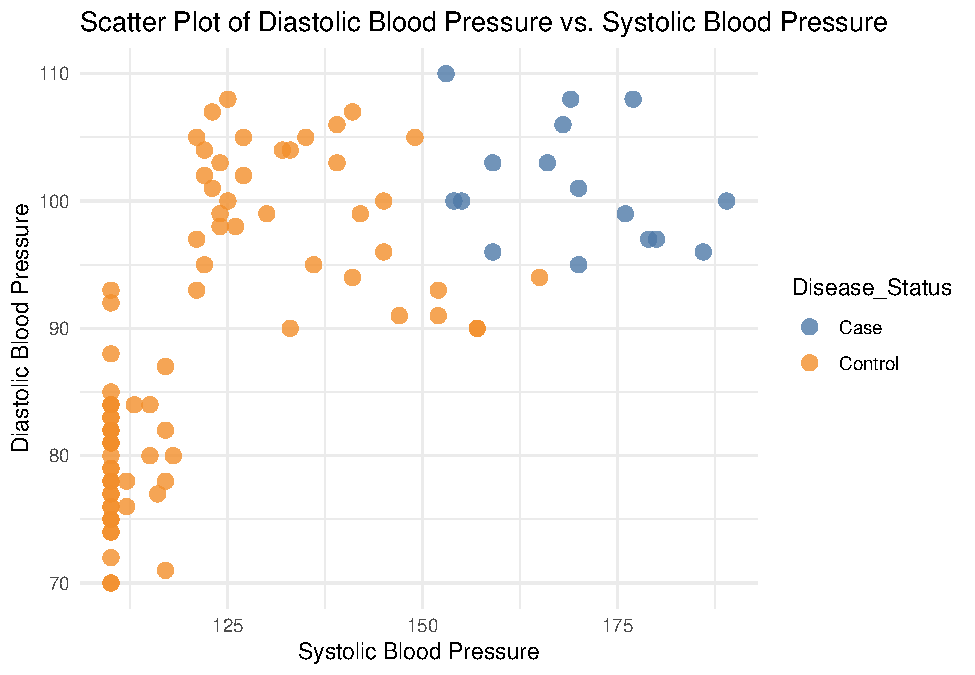
\includegraphics[keepaspectratio]{WeidnerSamuel-Assignment2_files/figure-latex/unnamed-chunk-5-1.pdf}}

\begin{enumerate}
\def\labelenumi{\arabic{enumi})}
\setcounter{enumi}{3}
\tightlist
\item
  Building off the code you used to generate the box plot above, add
  code that runs a wilcoxon rank sum test and display the resulting
  p-values comparing the cases and controls in the diastolic and
  systolic blood pressures on your box plot. Save your figure as a .png
  file and upload it with the submission for this assignment. After
  completing this, report the summary statistics for the systolic and
  diastolic blood pressures separately.
\end{enumerate}

\begin{Shaded}
\begin{Highlighting}[]
\DocumentationTok{\#\# Plan}
\CommentTok{\# 1. Define the png name for my boxplot output}
\CommentTok{\# 2. Add the same boxplot code as above, but add a stat\_compare\_means() function to pull the requested p values}
\CommentTok{\# 3. set the method to wilcox.test() for the wilcoxon rank sum test and explicitly define the grouping variable}
\CommentTok{\# 4. run dev.off() to output the boxplot in the png}
\CommentTok{\# 5. Add other wilcoxon test tables as a gut check the ggplot is pulling the correct p values for the right comparison}
\CommentTok{\# 6. Generate summary stats tables of the two BP variables}

\FunctionTok{png}\NormalTok{(}\StringTok{"bp\_boxplot.png"}\NormalTok{, }\AttributeTok{width =} \DecValTok{3000}\NormalTok{, }\AttributeTok{height =} \DecValTok{2000}\NormalTok{, }\AttributeTok{res =} \DecValTok{300}\NormalTok{) }\CommentTok{\# set png name and width and height so all is read correctly}

\FunctionTok{ggplot}\NormalTok{(long\_random\_data, }\FunctionTok{aes}\NormalTok{(}\AttributeTok{x =}\NormalTok{ blood\_pressure\_type, }\AttributeTok{y =}\NormalTok{ blood\_pressure\_reading, }\AttributeTok{fill =}\NormalTok{ Disease\_Status)) }\SpecialCharTok{+}
  \FunctionTok{geom\_boxplot}\NormalTok{() }\SpecialCharTok{+}
  \FunctionTok{labs}\NormalTok{(}\AttributeTok{x =} \StringTok{"Blood Pressure Type"}\NormalTok{, }\AttributeTok{y =} \StringTok{"Blood Pressure Value"}\NormalTok{, }\AttributeTok{fill =} \StringTok{"Disease Status"}\NormalTok{, }
       \AttributeTok{title =} \StringTok{"Blood Pressure Readings }\SpecialCharTok{\textbackslash{}n}\StringTok{by Type and Disease Status"}\NormalTok{) }\SpecialCharTok{+}
  \FunctionTok{theme\_minimal}\NormalTok{() }\SpecialCharTok{+}
  \FunctionTok{scale\_fill\_brewer}\NormalTok{(}\AttributeTok{palette =} \StringTok{"Set1"}\NormalTok{) }\SpecialCharTok{+}
  \FunctionTok{stat\_compare\_means}\NormalTok{(}\FunctionTok{aes}\NormalTok{(}\AttributeTok{group =}\NormalTok{ Disease\_Status), }\CommentTok{\# Add wilcoxon test and define grouping variable}
    \AttributeTok{method =} \StringTok{"wilcox.test"}
\NormalTok{  ) }

\FunctionTok{dev.off}\NormalTok{() }\CommentTok{\# output png}
\end{Highlighting}
\end{Shaded}

\begin{verbatim}
## pdf 
##   2
\end{verbatim}

\begin{Shaded}
\begin{Highlighting}[]
\NormalTok{wilcoxon\_summary\_stats\_sys }\OtherTok{\textless{}{-}} \FunctionTok{wilcox.test}\NormalTok{( }\DocumentationTok{\#\# Gut Check of systolic BP p value}
\NormalTok{  blood\_pressure\_reading }\SpecialCharTok{\textasciitilde{}}\NormalTok{ Disease\_Status,}
  \AttributeTok{data =} \FunctionTok{subset}\NormalTok{(long\_random\_data, blood\_pressure\_type }\SpecialCharTok{==} \StringTok{"Systolic\_Blood\_Pressure"}\NormalTok{)}
\NormalTok{)}

\FunctionTok{print}\NormalTok{(wilcoxon\_summary\_stats\_sys) }\CommentTok{\# Output }
\end{Highlighting}
\end{Shaded}

\begin{verbatim}
## 
##  Wilcoxon rank sum test with continuity correction
## 
## data:  blood_pressure_reading by Disease_Status
## W = 1333, p-value = 1.838e-10
## alternative hypothesis: true location shift is not equal to 0
\end{verbatim}

\begin{Shaded}
\begin{Highlighting}[]
\NormalTok{wilcoxon\_summary\_stats\_diast }\OtherTok{\textless{}{-}} \FunctionTok{wilcox.test}\NormalTok{( }\DocumentationTok{\#\# Gut Check of diastolic BP p value}
\NormalTok{  blood\_pressure\_reading }\SpecialCharTok{\textasciitilde{}}\NormalTok{ Disease\_Status,}
  \AttributeTok{data =} \FunctionTok{subset}\NormalTok{(long\_random\_data, blood\_pressure\_type }\SpecialCharTok{==} \StringTok{"Diastolic\_Blood\_Pressure"}\NormalTok{)}
\NormalTok{)}

\FunctionTok{print}\NormalTok{(wilcoxon\_summary\_stats\_diast) }\CommentTok{\# Output }
\end{Highlighting}
\end{Shaded}

\begin{verbatim}
## 
##  Wilcoxon rank sum test with continuity correction
## 
## data:  blood_pressure_reading by Disease_Status
## W = 1107.5, p-value = 4.269e-05
## alternative hypothesis: true location shift is not equal to 0
\end{verbatim}

\begin{Shaded}
\begin{Highlighting}[]
\NormalTok{systolic\_summary\_stats }\OtherTok{\textless{}{-}}\NormalTok{ long\_random\_data }\SpecialCharTok{\%\textgreater{}\%} \CommentTok{\# Summary stats for systolic BP using summarise()}
  \FunctionTok{filter}\NormalTok{(blood\_pressure\_type }\SpecialCharTok{==} \StringTok{"Systolic\_Blood\_Pressure"}\NormalTok{) }\SpecialCharTok{\%\textgreater{}\%}
  \FunctionTok{summarise}\NormalTok{(}\StringTok{"Number of Participants"} \OtherTok{=} \FunctionTok{n\_distinct}\NormalTok{(Participant\_ID), }\CommentTok{\# number of participants vs. readings}
            \StringTok{"Count Observations"} \OtherTok{=} \FunctionTok{n}\NormalTok{(),}
            \StringTok{"Mean Systolic Blood Pressure"} \OtherTok{=} \FunctionTok{mean}\NormalTok{(blood\_pressure\_reading),}
            \StringTok{"Median Systolic Blood Pressure"} \OtherTok{=} \FunctionTok{median}\NormalTok{(blood\_pressure\_reading),}
            \StringTok{"Max Systolic Blood Pressure"} \OtherTok{=} \FunctionTok{max}\NormalTok{(blood\_pressure\_reading),}
            \StringTok{"Min Systolic Blood Pressure"} \OtherTok{=} \FunctionTok{min}\NormalTok{(blood\_pressure\_reading),}
            \StringTok{"IQR Systolic Blood Pressure"} \OtherTok{=} \FunctionTok{IQR}\NormalTok{(blood\_pressure\_reading) }\CommentTok{\# diff between 25th and 75th percentile}
\NormalTok{  )}

\FunctionTok{print}\NormalTok{(systolic\_summary\_stats) }\CommentTok{\# output}
\end{Highlighting}
\end{Shaded}

\begin{verbatim}
## # A tibble: 1 x 7
##   `Number of Participants` `Count Observations` `Mean Systolic Blood Pressure`
##                      <int>                <int>                          <dbl>
## 1                      100                  100                           129.
## # i 4 more variables: `Median Systolic Blood Pressure` <dbl>,
## #   `Max Systolic Blood Pressure` <dbl>, `Min Systolic Blood Pressure` <dbl>,
## #   `IQR Systolic Blood Pressure` <dbl>
\end{verbatim}

\begin{Shaded}
\begin{Highlighting}[]
\NormalTok{diastolic\_summary\_stats }\OtherTok{\textless{}{-}}\NormalTok{ long\_random\_data }\SpecialCharTok{\%\textgreater{}\%} \CommentTok{\# Summary stats for diastolic BP using summarise()}
  \FunctionTok{filter}\NormalTok{(blood\_pressure\_type }\SpecialCharTok{==} \StringTok{"Diastolic\_Blood\_Pressure"}\NormalTok{) }\SpecialCharTok{\%\textgreater{}\%}
  \FunctionTok{summarise}\NormalTok{(}\StringTok{"Number of Participants"} \OtherTok{=} \FunctionTok{n\_distinct}\NormalTok{(Participant\_ID), }\CommentTok{\# number of participants vs. readings}
            \StringTok{"Count Observations"} \OtherTok{=} \FunctionTok{n}\NormalTok{(),}
            \StringTok{"Mean Diastolic Blood Pressure"} \OtherTok{=} \FunctionTok{mean}\NormalTok{(blood\_pressure\_reading),}
            \StringTok{"Median Diastolic Blood Pressure"} \OtherTok{=} \FunctionTok{median}\NormalTok{(blood\_pressure\_reading),}
            \StringTok{"Max Diastolic Blood Pressure"} \OtherTok{=} \FunctionTok{max}\NormalTok{(blood\_pressure\_reading),}
            \StringTok{"Min Diastolic Blood Pressure"} \OtherTok{=} \FunctionTok{min}\NormalTok{(blood\_pressure\_reading),}
            \StringTok{"IQR Diastolic Blood Pressure"} \OtherTok{=} \FunctionTok{IQR}\NormalTok{(blood\_pressure\_reading) }\CommentTok{\# diff between 25th and 75th percentile}
\NormalTok{  )}

\FunctionTok{print}\NormalTok{(diastolic\_summary\_stats) }\CommentTok{\# output}
\end{Highlighting}
\end{Shaded}

\begin{verbatim}
## # A tibble: 1 x 7
##   `Number of Participants` `Count Observations` `Mean Diastolic Blood Pressure`
##                      <int>                <int>                           <dbl>
## 1                      100                  100                            90.2
## # i 4 more variables: `Median Diastolic Blood Pressure` <dbl>,
## #   `Max Diastolic Blood Pressure` <dbl>, `Min Diastolic Blood Pressure` <dbl>,
## #   `IQR Diastolic Blood Pressure` <dbl>
\end{verbatim}

\begin{enumerate}
\def\labelenumi{\arabic{enumi})}
\setcounter{enumi}{4}
\tightlist
\item
  Remove the systolic and diastolic blood pressure columns in the wide
  format data frame. Generate a heart rate column instead and add that
  to the data frame. The heart rates should be dependent on the level of
  activity of the participant. Participants who are ``Inactive'' should
  have a heart rate taken from a normal distribution with a minimum of
  100 and a maximum of 200. The mean of this distribution should be 150
  and have a standard deviation of 20. If the participant is ``Lightly
  Active'', their heart rate should be taken from a normal distribution
  with a minimum of 80 and a maximum of 99. The mean of this
  distribution should be 85 and the standard deviation should be 20.
  Finally, if the participant is ``Average Activity'' or ``Very
  Active,'' their heart rate should be taken from a normal distribution
  with a minimum of 40 and a maximum of 70. The mean of this
  distribution should be 50 and the standard deviation 20.
\end{enumerate}

\begin{Shaded}
\begin{Highlighting}[]
\DocumentationTok{\#\# Plan}
\CommentTok{\# 1. create a new data frame, set it to the original wide data}
\CommentTok{\# 2. use the pipe operator to manipulate it, removing the BP columns}
\CommentTok{\# 3. group by activity status and mutate based on a conditional that evaluates based on group status to the specific sampling requested}
\CommentTok{\# 4. show the first few rows of the data}

\NormalTok{random\_data\_heart\_rate }\OtherTok{\textless{}{-}}\NormalTok{ random\_data }\SpecialCharTok{\%\textgreater{}\%}
  \FunctionTok{select}\NormalTok{(}\SpecialCharTok{{-}}\NormalTok{Systolic\_Blood\_Pressure, }\SpecialCharTok{{-}}\NormalTok{Diastolic\_Blood\_Pressure) }\SpecialCharTok{\%\textgreater{}\%} \CommentTok{\# remove bp columns}
  \FunctionTok{group\_by}\NormalTok{(Activity\_Status) }\SpecialCharTok{\%\textgreater{}\%} \CommentTok{\# group by activity status}
  \CommentTok{\# Run the specific sampling pattern depending on the activity status group}
  \FunctionTok{mutate}\NormalTok{(}
    \AttributeTok{Heart\_Rate =} \ControlFlowTok{if}\NormalTok{ (}\FunctionTok{cur\_group}\NormalTok{()}\SpecialCharTok{$}\NormalTok{Activity\_Status }\SpecialCharTok{==} \StringTok{"Inactive"}\NormalTok{) \{ }\CommentTok{\# use a conditional to determine which sampling pattern}
      \FunctionTok{pmax}\NormalTok{(}\DecValTok{100}\NormalTok{, }\FunctionTok{pmin}\NormalTok{(}\DecValTok{200}\NormalTok{, }\FunctionTok{round}\NormalTok{(}\FunctionTok{rnorm}\NormalTok{(}\FunctionTok{n}\NormalTok{(), }\AttributeTok{mean =} \DecValTok{150}\NormalTok{, }\AttributeTok{sd =} \DecValTok{20}\NormalTok{))))}
\NormalTok{    \} }\ControlFlowTok{else} \ControlFlowTok{if}\NormalTok{ (}\FunctionTok{cur\_group}\NormalTok{()}\SpecialCharTok{$}\NormalTok{Activity\_Status }\SpecialCharTok{==} \StringTok{"Lightly Active"}\NormalTok{) \{}
      \FunctionTok{pmax}\NormalTok{(}\DecValTok{80}\NormalTok{, }\FunctionTok{pmin}\NormalTok{(}\DecValTok{99}\NormalTok{, }\FunctionTok{round}\NormalTok{(}\FunctionTok{rnorm}\NormalTok{(}\FunctionTok{n}\NormalTok{(), }\AttributeTok{mean =} \DecValTok{85}\NormalTok{, }\AttributeTok{sd =} \DecValTok{20}\NormalTok{))))}
\NormalTok{    \} }\ControlFlowTok{else}\NormalTok{ \{}
      \FunctionTok{pmax}\NormalTok{(}\DecValTok{40}\NormalTok{, }\FunctionTok{pmin}\NormalTok{(}\DecValTok{70}\NormalTok{, }\FunctionTok{round}\NormalTok{(}\FunctionTok{rnorm}\NormalTok{(}\FunctionTok{n}\NormalTok{(), }\AttributeTok{mean =} \DecValTok{50}\NormalTok{, }\AttributeTok{sd =} \DecValTok{20}\NormalTok{))))}
\NormalTok{    \} }
\NormalTok{  ) }\SpecialCharTok{\%\textgreater{}\%}
  \FunctionTok{ungroup}\NormalTok{()}

\FunctionTok{head}\NormalTok{(random\_data\_heart\_rate) }\CommentTok{\# show first few rows of the data}
\end{Highlighting}
\end{Shaded}

\begin{verbatim}
## # A tibble: 6 x 6
##   Participant_ID Sex      Age Activity_Status Disease_Status Heart_Rate
##   <chr>          <chr>  <dbl> <chr>           <chr>               <dbl>
## 1 pt_1           Male      53 Lightly Active  Case                   80
## 2 pt_2           Male      50 Lightly Active  Case                   90
## 3 pt_3           Male      50 Inactive        Control               186
## 4 pt_4           Female    64 Lightly Active  Control                80
## 5 pt_5           Male      48 Inactive        Control               156
## 6 pt_6           Female    65 Inactive        Control               153
\end{verbatim}

\end{document}
